\chapter{Introduction}


\vspace{2mm}

\section{Motivation}
\textbf{Author: Sztavinovszki}
In almost every robotics application nowadays you need some kind of communication. Wether it is a robot communicating
its data to a home-base, or two robots sharing data with one another. Over the past years communication has drastically
improved with new protocols and technology, such as Bluetooth Low energy.

\section{Goal}
\textbf{Author: Sztavinovszki}

\section{History}
\textbf{Author: Dragosits}
The history of communication and coordination between seperate systems is long and extensive. Nowadays it is an essential 
function of almost every technological device. In the field of computing it started in the late 1950s with SAGE (Semi-Automatic Ground Enviornment),
which was a network of computers and networking technology created by the United States of America military, 
and it allowed the transfer of radar data nation-wide.[]
%Haigh, Thomas; Ceruzzi, Paul E. (14 September 2021). A New History of Modern Computing. MIT Press. pp. 87–89. ISBN 978-0262542906.
The next major step forward was the beginning of ARPANET in 1969, which served as a connection between multiple north american 
universities, and laid the groundwork for the modern internet.[] 
In more recent times is the internet of things commonplace, and is used for the interchange of terabytes of data each day.

\section{Project Management}
\textbf{Author: Sztavinovszki}

\section{Outline}
%\section{Section}
%More text. \lipsum[1] See Figure~\ref{pic:example}.

%\begin{figure}[h]
%	\centering
%	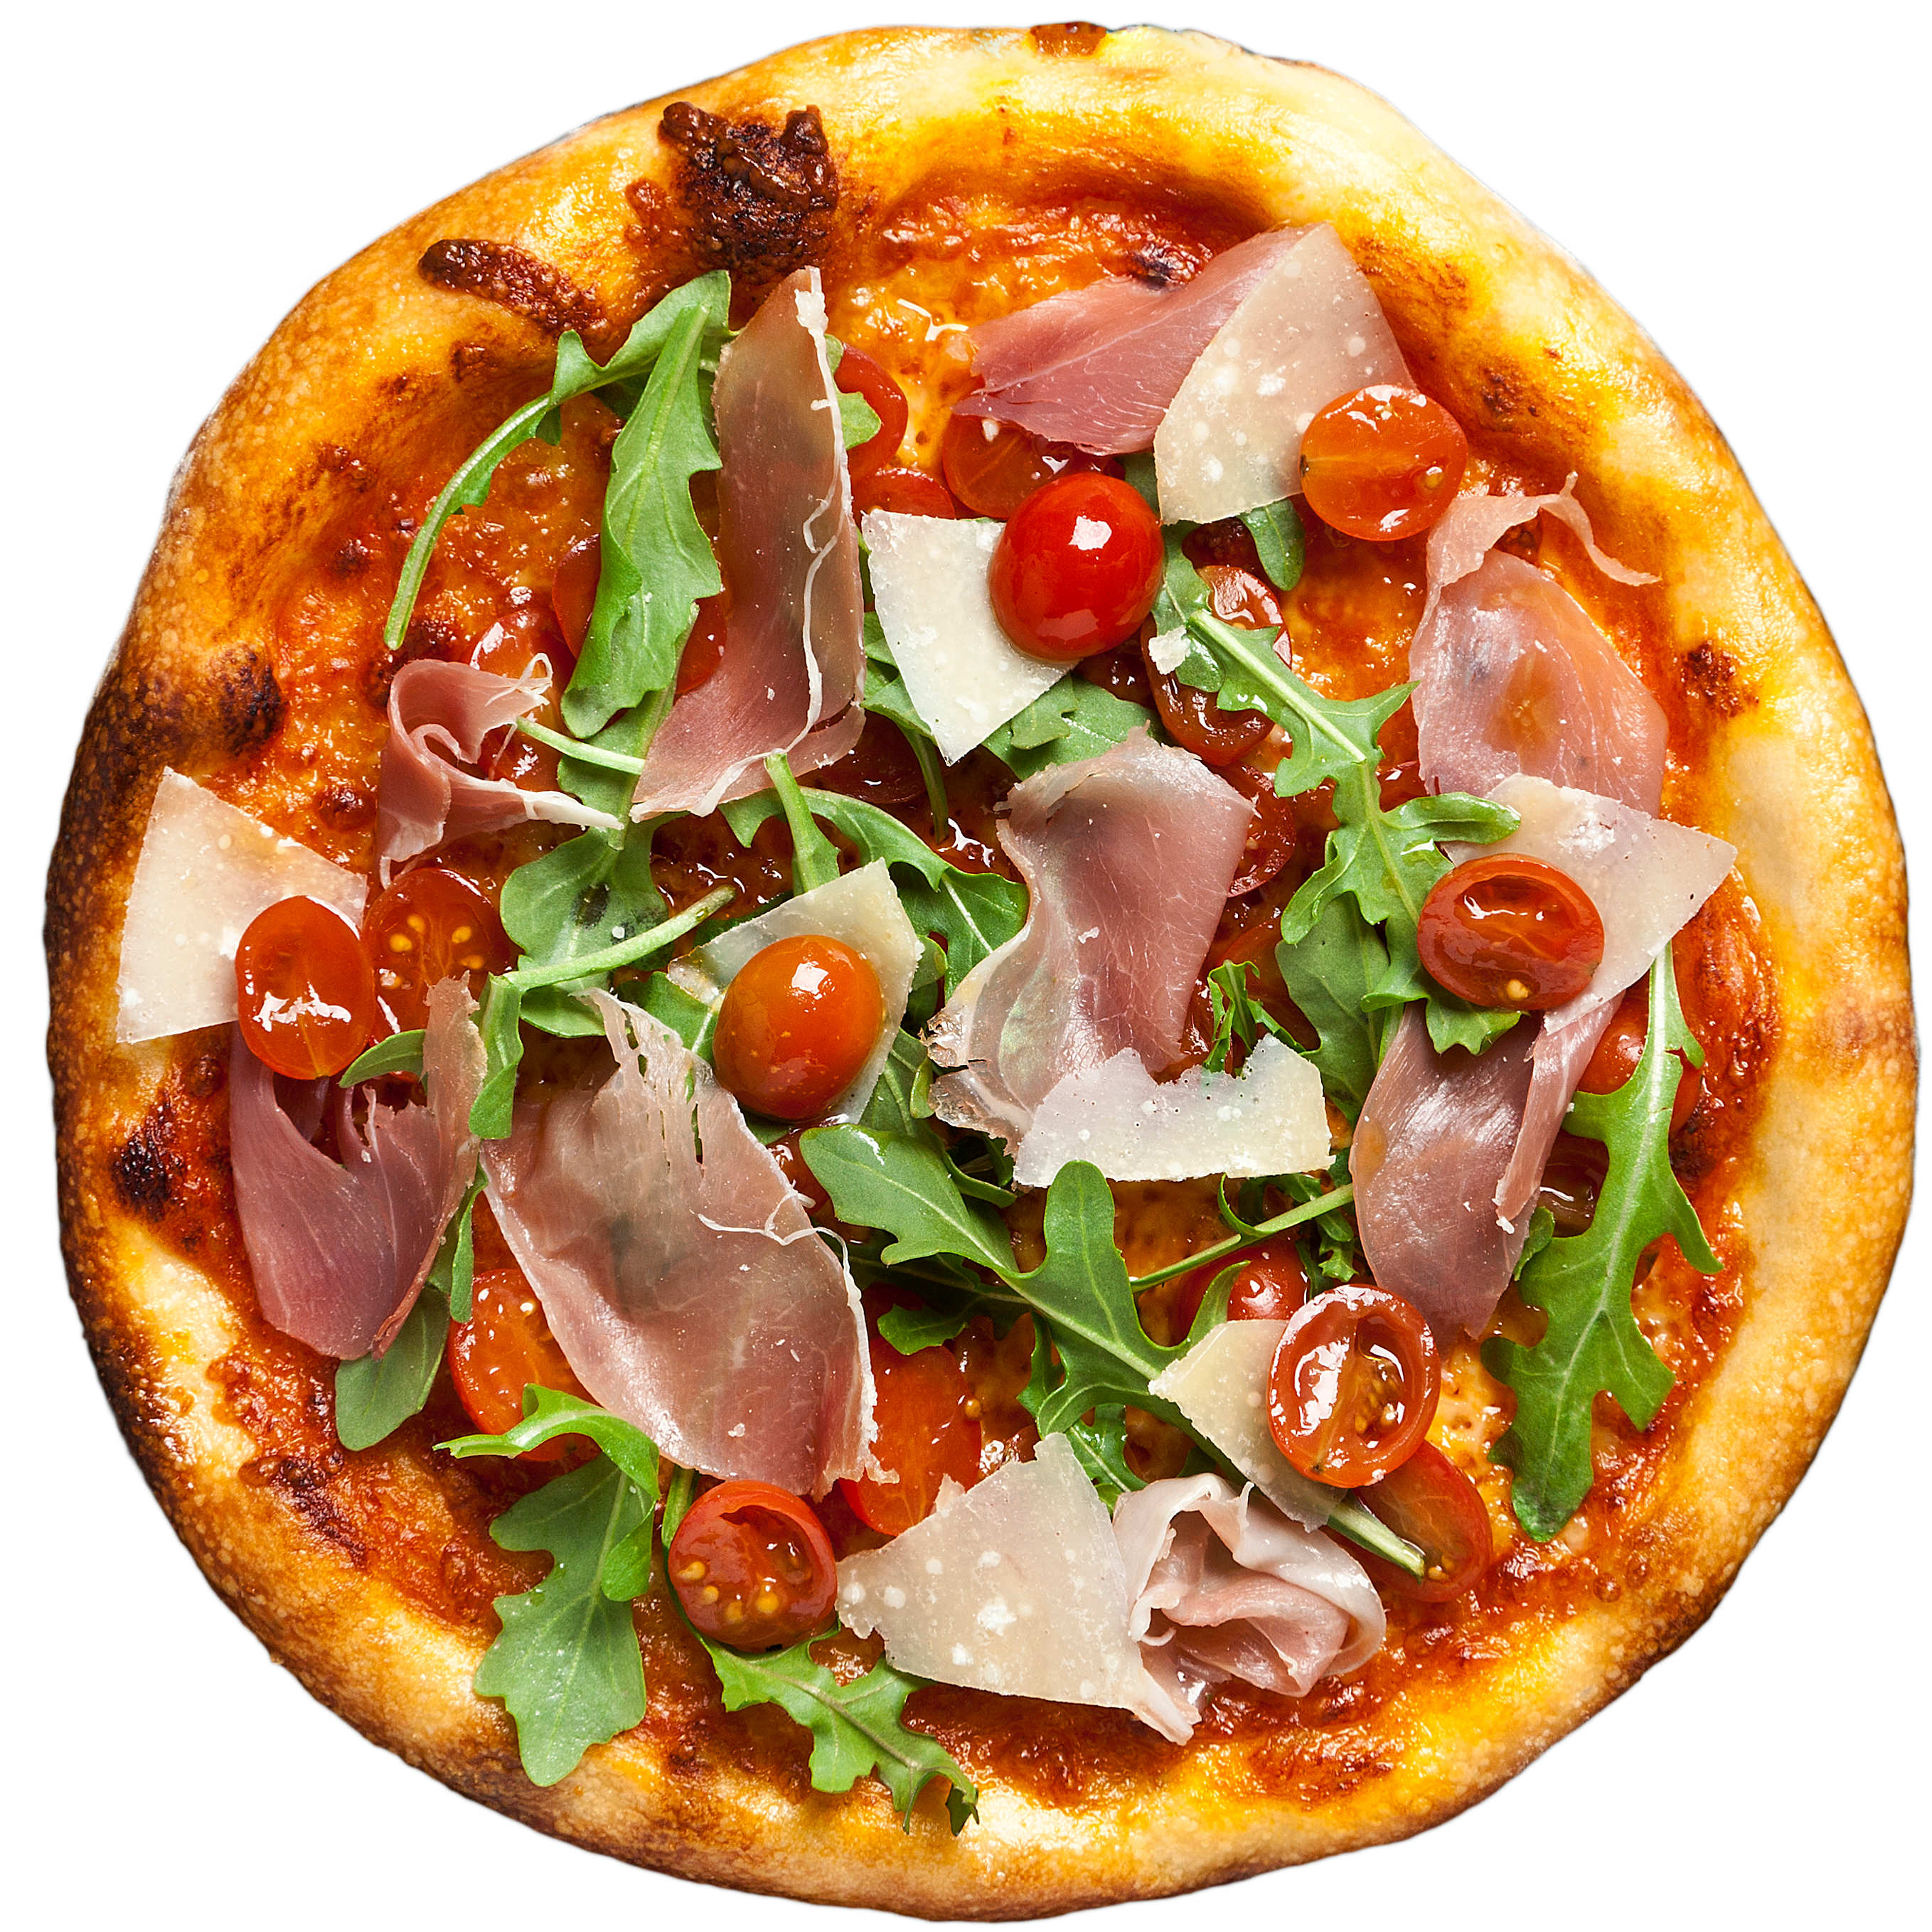
\includegraphics[width=2.5in]{img/example.png}
%	\caption{Picture description.}
%	\label{pic:example}
%\end{figure}

%\subsection{Subsection}
%\lipsum[1]

%\subsection{Subsection}
%\lipsum[1] See Table~\ref{tab:example}.

%\begin{center}
%	\begin{tabular}{| l | l | l |}
%		\hline
%		\bfseries Header 1 & \bfseries Header 2 & \bfseries Header 2 \\
%		\hline
%		Text & text & text \\
%		\hline
%		Text & text & text  \\
%		\hline
%		Text & text & text  \\
%		\hline
%	\end{tabular}
%	\label{tab:example}
%\end{center}

%\lipsum[1] Some references can be found at \footcite{robo4you} or at \footcite{Hope_Learning_TensorFlow}.
%

\filbreak
